\chapter{Démonstration pour l'analyse descriptive sur un grand corpus}
\label{chap:demo}
Ce chapitre décrit le processus et les résultats observés lors de l'application de la chaîne proposée (Figure \ref{fig:intro:pipeline-globale}) sur un corpus formé de la base CAPP de la \citet{dila2019capp} (+65k XML sur 1997-2019), une base du tribunal de commerce de Paris (300k MS DOC sur ?-?) et plus de 500k décisions collectées de Legifrance. Le module d'extraction d'information (Figure \ref{fig:demo:module-extraction}) est un système qui comprend les modèles développés durant les expérimentations de cette thèse. 
%à CAPP\_20190805-214041.tar.gz et Freemium_capp\_global\_20180315-170000.tar.gz 

%\verb|wget -c --accept='*.tar.gz' -r  ftp://echanges.dila.gouv.fr/CAPP/|

\begin{figure}[!htb]
	\centering 
	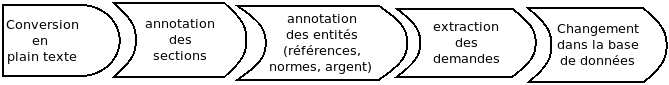
\includegraphics[width=0.8\textwidth]{pipeline-demo.png}
	\caption{Détails du module d'extraction d'information}\label{fig:demo:module-extraction}
\end{figure}

% répartition par ville?

\section{Illustration d'analyses descriptives}
\label{sec:demo:experimentations}

bkjbj


\subsection{Implémentation du système}

bkjbj;


\subsection{Données}
\subsubsection{Distribution de la base dans l'espace et dans le temps}

Données de la base CAP (64733 docs de la période 1997-2018 CA et 1er jugements) + scrapping de LegiFrance (? cour d'appel + ? 1er jugements) +  (300k Tribunal de commerce de paris)


\subsection{Analyse du sens du résultat}
;bkjkl
\subsubsection{Evolution dans le temps}
\subsubsection{Différence dans l'espace}

\subsection{Analyse des quanta}
,bkjlihio
\subsubsection{Evolution dans le temps}
\subsubsection{Différence dans l'espace}
\subsubsection{Quantum demandé vs. quantum accordé}

\section{Conclusion}
\label{sec:demo:conclusion}
hgfgh
lkhk